\documentclass[
	article,
    a4paper,
    12pt,
    oneside,
    english,			% idioma adicional para hifenização
    brazil,
    sumario=tradicional
]{abntex2}

% Packages
\usepackage[T1]{fontenc}		% Selecao de codigos de fonte.
\usepackage[utf8]{inputenc}		% Codificacao do documento (conversão automática dos acentos)
\usepackage{indentfirst}		% Indenta o primeiro parágrafo de cada seção.
\usepackage{nomencl} 			% Lista de simbolos
\usepackage{color}				% Controle das cores
\usepackage{graphicx}			% Inclusão de gráficos
\graphicspath{{src/assets/}}  % Local das imagens
\usepackage{subfig}
\usepackage{microtype} 			% para melhorias de justificação

% Pacotes de citações
%\usepackage[brazilian,hyperpageref]{backref}	 % Paginas com as citações na bibl
\usepackage[alf]{abntex2cite}	% Citações padrão ABNT
% End Packages

% Configurando margens
\setlrmarginsandblock{3cm}{2cm}{*} % margem esquerda e direita
\setulmarginsandblock{3cm}{2cm}{*} % margem superior e inferior
\checkandfixthelayout

% Meta
\title{WEB EM TEMPO REAL \\Soluções para comunicação em tempo real entre clientes e servidores.}
\author{Iosley Carlos Silva}
\date{\today}
% End Meta

% Informações do PDF
\makeatletter
\hypersetup{
	%pagebackref=true,
	pdftitle={\@title}, 
	pdfauthor={\@author},
	pdfsubject={\@title},
	pdfcreator={LaTeX with abnTeX2},
	pdfkeywords={atigo científico}, 
	colorlinks=true,       		% false: boxed links; true: colored links
	linkcolor=black, 			% color of internal links
	citecolor=black, 			% color of links to bibliography
	filecolor=black, 		 % color of file links
	urlcolor=black,
	bookmarksdepth=4
}
% --- 
% Espaçamentos entre linhas e parágrafos 
% --- 

% O tamanho do parágrafo é dado por:
\setlength{\parindent}{1.25cm}

% Controle do espaçamento entre um parágrafo e outro:
\setlength{\parskip}{0.2cm}  % tente também \onelineskip

\begin{document}
	
\maketitle

{
	\small
	\ignorespacesafterend
	\noindent

	\textbf{Resumo}:
	% Introdução
	Em poucos anos após a sua criação, a World Wide Web passou de páginas estática e não interativa para aplicações ricas e complexas. Estas mudanças foram acompanhadas da melhoria dos ambientes de execução e tecnologias de desenvolvimento. A medida que as aplicações web se tornaram mais dinâmicas, com um alto volume de mensagens trocadas entre clientes e servidores, foi se fazendo necessário o uso de técnicas para reduzir a latência e permitir uma comunicação mais atempada.
	% Objetivo:
	% O objetivo é em geral a informação de maior interesse: qual o objetivo dos autores com esse estudo? Por esse motivo, a primeira frase do artigo deve conter, na minha opinião, o objetivo do estudo, também chamado statement of purpose: “O objetivo deste estudo é…”, “Neste artigo propomos…”, etc.
	Este estudo tem por objetivo compreender as limitações do protocolo HTTP para comunicação em tempo real na web, exibir métodos paliativos no contexto histórico e soluções atualmente utilizadas para desenvolvimento de aplicações web que exijam uma comunicação constante entre cliente e servidor,
	% Materiais e métodos:
	% Com esse objetivo em mente, como os autores propõem atacar o problema? O resumo deve, portanto, dar uma breve descrição da metodologia usada para atingir o objetivo proposto.
	através de uma pesquisa documental com a utilização de materiais teóricos que abordam o tema e desenvolvem conceitos, ideias e entendimentos, visando buscar soluções, e compreender os pontos positivos e negativos de cada solução.
	% Resultados:
	% Deve-se naturalmente apresentar os principais resultados de forma resumida e concreta, através de informações quantitativas úteis em lugar de afirmações vagas de valor dúbio.
	Demonstrar as capacidades e limitações do AJAX, as vantagens da utilização das APIs de Server-Sent Event e WebSockets nos navegadores modernos,
	% Conclusões:
	% Por fim, quais são as conclusões do estudo? Qual a relevância dos resultados apresentados? Como os resultados avançam o conhecimento na área ou ajudam a resolver o problema proposto?
	confirmando que, por ter baixa latência e boa aceitação por parte dos navegadores modernos, o WebSockets se mostra como a melhor solução para a comunicação bi-direcional entre um cliente e servidor, permitindo a comunicação por um único soquete TCP operando na mesma porta padrão do HTTP
	
	\vspace{\onelineskip}

	\textbf{Palavras-chave}: Ajax. XHR. SSE. WebSockets.
}
{
	\small
	\noindent
	
	\textbf{Abstract}:
	In a few years after its creation, the World Wide Web has gone from static and non-interactive pages to rich and complex applications. These changes were accompanied by improved execution environments and development technologies. As web applications became more dynamic, with a high amount of messages exchanged between clients and servers, it became necessary to use techniques to reduce latency and allow a more timely communication. This study aims to understand the limitations of the HTTP protocol for real-time communication on the web, to display palliative methods in the historical context and solutions currently used for web application development that require constant communication between client and server, through documentary research with use of theoretical materials that approach the theme and develop concepts, ideas and understandings, aiming to find solutions, and understand the positives and negatives of each solution. Demonstrate the capabilities and limitations of AJAX, the advantages of using the Server-Sent Event and WebSockets in modern browsers. Afirm that, because of the low latency and good acceptance of the modern browsers, WebSockets proves to be the best solution for two-way communication between a client and server, allowing communication over a single TCP socket operating on the same standard HTTP port
	
	\vspace{\onelineskip}
	
	\textbf{Keywords}: Ajax. XHR. SSE. WebSockets.
}

\section{INTRODUÇÃO}

% Focaliza-se a “questão” na literatura para indicar a originalidade e relevância do trabalho, a metodologia utilizada na pesquisa, bem como identificar os objetivos do estudo no ultimo parágrafo.

A internet\footnote{Conjunto mundial de redes de computadores.} como é hoje passou por diversas transformações com a melhoria dos hardwares\footnote{Parte física de um computador} necessários para seu funcionamento e a definição de protocolos formais para a intercomunicação entre diversos dispositivos \cite{Aghaei2012}.

Porem, a transformação mais notável desde então, foi no tratamento dos dados. Hoje as informações estão acessíveis de qualquer lugar do mundo, isto trouxe também um aumento na retenção da informação e uma mudança drástica na maneira de manipular e transmitir estas informações \cite{Leiner2009}.

Hoje as páginas web são mais dinâmicas podendo ser desenvolvidas aplicações modernas, que antes precisavam ser instaladas no computador, rodando direto do navegador\footnote{Programa de computador que possibilita a interação com documentos virtuais da Internet.},  proporcionando a mesma experiência experimentada com as aplicações nativas \cite{Garrett2005}.

Para ter uma experiência fluida nestas aplicações, os navegadores precisam se comunicar com os servidores\footnote{Sistema de computação centralizada que fornece serviços a uma rede de computadores.} de maneira rápida e eficiente. Para isto, são usadas técnicas para a transmissão e recebimento de informações em tempo real. Estas técnicas mantem as informações sincronizadas entra a aplicação cliente e o servidor de maneira transparente para o usuário \cite{offutt2002quality}.

Estes avanços proporcionaram uma participação muito maior dos usuários que agora deixam de ser meros consumidores de conteúdo e passam a ser os maiores produtores de conteúdo multimídia \cite{Aghaei2012}.

No entanto, entende-se que mudanças foram necessárias para acompanhar esta evolução. Mudanças que pudessem coexistir com a maneira já existente de transmissão de dados ao passo que tornasse mais eficiente e mais rápida a transmissão da informação.



\section{REFERENCIAL TEÓRICO}

Em agosto de 1962, foi previsto um conjunto global interconectado de computadores através do qual todos poderiam acessar dados e programas, descrito em memorandos escritos por J.C.R. Licklider do MIT\footnote{Instituto de Tecnologia de Massachusetts é uma universidade privada de pesquisa localizada em Cambridge, Massachusetts, Estados Unidos.} quando este discutiu sobre o conceito de “Rede Galáctica”, conceito este muito semelhante com a internet de hoje \cite[p.~2]{Leiner2009}.

Para a intercomunicação de computadores de diferentes fabricantes, se fez necessário uma arquitetura aberta que foi primariamente introduzida por Kahn Shortly da DARPA\footnote{Agência de Projetos de Pesquisa Avançada de Defesa dos Estados Unidos.} em 1972 com o \emph{Netware Core Protocol} (NCP), um protocolo para comunicação bi-direcional identificada por um par de números de soquetes\footnote{Mecanismo de comunicação que permite a troca de mensagens entre os processos de uma máquina/aplicação servidor e uma máquina/aplicação cliente.} \cite[p.~4]{Leiner2009}.

Sucedendo e substituindo o protocolo NCP, o Protocolo de Controle de Transmissão (TCP)\footnote{Padrão que define como estabelecer e manter uma conversa de rede através da qual os programas de aplicativos podem trocar dados.}, vinha sendo implementado desde 1980 mas foi somente em 1983 que a transição definitiva aconteceu, exigindo que todos os \emph{hosts}\footnote{É qualquer máquina ou computador conectado a uma rede, podendo oferecer informações, recursos, serviços e aplicações aos usuários ou outros nós na rede.} convertessem simultaneamente para que continuassem funcionando \cite[p.~7]{Leiner2009}.

Nesta época, já era possível via Internet, entrar em sessões com máquinas remotas e trocar mensagens, porem, de acordo com \citeonline{Aghaei2012}, somente em 1989, Tim Berners-Lee sugere a criação de um espaço de hipertexto\footnote{Apresentação de informações, organizada de tal maneira que o leitor tem liberdade de escolher vários caminhos, a partir de sequências associativas possíveis entre blocos vinculados por remissões, sem estar preso a um encadeamento linear único.} global na qual qualquer informação acessível seria referida por um único Identificador de Documento Universal (UDI), este espaço seria posteriormente conhecido por Word Wide Web (WWW) ou simplesmente Web.

Em 1991 Tim Berners-Lee do CERN\footnote{Organização Europeia para a Pesquisa Nuclear, é o maior laboratório de física de partículas do mundo.}, na Suíça, apresentou um novo sistema de informação baseado na Internet (WWW) tornando-se possível criar servidores de informação, onde se incluem textos, imagens e multimédia \cite{goethals2000historia}.

Segundo \citeonline{Aghaei2012}, as principais tecnologias da Web eram:
\begin{description}
	\item[Hypertext Markup Language (HTML)] que segundo \citeonline{Berners-Lee1993}: é uma linguagem de marcação usada para criar documentos de hipertexto;

	\item[Identificador Uniforme de Recurso (URI)]  que segundo \citeonline{Connolly2000}: é o identificador de fragmento que designa o elemento com o nome correspondente;

	\item[Protocolo de Transferência de Hipertexto (HTTP)] que segundo \citeonline[p.~7]{Fielding1999}: “O HTTP é um protocolo de nível de aplicação para sistemas de informação distribuídos, colaborativos e hipermídia”.
\end{description}

\subsection{O protocolo HTTP}
Em uso desde 1990, teve sua primeira versão referida como HTTP / 0.9. Era um protocolo simples para transferência de dados através da internet. A partir da versão 1.0, o protocolo foi melhorado permitindo modificadores sobre a semântica “requisição / resposta” para que duas aplicações determinassem as capacidades verdadeiras de cada uma \cite[p.~7]{Fielding1999}.

No modelo HTTP padrão, um servidor não inicia uma conexão com um cliente, enviando respostas somente quando solicitado. Assim, não é possível que um servidor envie eventos assíncronos para aplicações clientes, forçando o cliente à pesquisar periodicamente por novos conteúdos no servidor, o que consome uma quantidade significativa de trafego de dados e reduz a capacidade de resposta da aplicação, pois o servidor precisa ser requisitado para enviar as atualizações \cite{Loreto2011}.

\begin{figure}[!htb]
	\centering
	\caption{Modelo de requisição HTTP}
	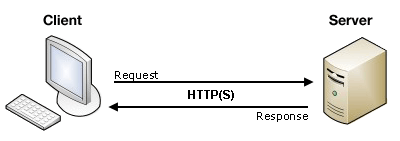
\includegraphics[width=350px]{http.png}
	\fonte{\citeonline{Mills2017mozilla}}
	\label{HTTP}
\end{figure}

\subsection{A Evolução da WEB}
A Web no inicio era somente leitura, estática e mono-direcional. O principal objetivo era publicar informações para e estabelecer uma presença on-line. Os sites\footnote{Local na Internet identificado por um nome de domínio, constituído por uma ou mais páginas de hipertexto.} eram estáticos e não interativos. Os Usuários não poderiam fazer contribuições nem interagir com os sites, sendo estes meros panfletos digitais \cite[p.~2-3]{Aghaei2012}.

A medida que as os desenvolvedores começaram a criar páginas cada vez mais dinâmicas, foi se fazendo necessário o uso de técnicas para melhorar a comunicação. Em 1999 quando o Internet Explorer 5\footnote{Uma série de navegadores web gráficos desenvolvidos pela Microsoft.} implementou o AJAX\footnote{Técnicas para programação que utilizam tecnologias como JavaScript e XML para carregar informações de forma assíncrona.} pela primeira vez \cite{Asleson2006}, as páginas web já podiam ser muito mais flexíveis e rápidas, já não era mais preciso sair da página para buscar informação no servidor, mas ainda não havia uma maneira do servidor enviar mensagens espontaneamente para o cliente.

\subsection{Soluções paliativas}

Várias técnicas foram implementadas nos últimos anos para permitir que um servidor web envie atualizações para clientes Dentre as principais, destacam-se:

\begin{description}
	\item[HTTP Polling:] Consiste de uma sequencia de requisições que o cliente emite para o servidor com intervalo determinado, recebendo uma resposta vazia caso novas mensagens não estejam disponíveis \cite{Pimentel2012}.

	\item[Long Polling HTTP:] O servidor tenta “manter aberta” (não responder imediatamente) a cada solicitação HTTP, respondendo apenas quando há novos dados para entregar. Desta forma, existe sempre um pedido pendente ao qual o servidor pode responder com o objectivo de disparar eventos à medida que ocorrem, minimizando assim a latência na entrega de mensagens \cite{Aghaei2012}.

	\item[HTTP Streaming\footnote{Tecnologia que envia informações multimídia, através da transferência de dados, utilizando redes de computadores.}:] O servidor mantém uma solicitação aberta indefinidamente, ou seja, nunca finaliza a resposta ou fecha a conexão, mesmo depois de enviar dados para o cliente.
\end{description}

Segundo \citeonline[p.~3]{Loreto2011}, “Esses mecanismos podem fornecer atualizações aos clientes de forma mais atempada, evitando a latência experimentada pelas aplicações clientes devido à frequente abertura e fechamento de conexões necessárias para periodicamente pesquisar dados”.

É importante entender que estas soluções nem sempre são eficazes e para alguns casos uma busca periódica pode até ser mais eficiente, como é o exemplo de aplicações com alto volume de mensagens, onde o Long Polling não oferece melhorias de desempenho se comparado a sondagem tradicional porque a reconexão é constante \cite{Wang2013}.

Já o Streaming, mesmo sendo uma grande solução, entrega mensagens de maneira imprevisível. Alguns proxies\footnote{Intermediários entre o usuário e seu servidor.} e firewalls\footnote{Dispositivo de segurança da rede que monitora o tráfego de rede de entrada e saída e decide permitir ou bloquear tráfegos específicos de acordo com um conjunto definido de regras de segurança.} podem guardar em memória a resposta o que pode resultar em uma maior latência, não sendo recomenda para redes onde existam firewalls ou proxies \cite[p.~6]{Wang2013}.

\subsection{Soluções atuais}

Para eliminar estes problemas, a sessão de conexão do HTML5\footnote{Quinta versão da linguagem HTML.} inclui o WebSocket. Segundo \citeonline[p.~47, Tradução~nossa]{Pimentel2012}, “O protocolo WebSocket fornece um canal de comunicação bi-direcional, que opera através de um único soquete e pode ajudar a criar aplicativos escaláveis em tempo real na Web”.

O protocolo consiste de um handshake\footnote{Processo pelo qual duas máquinas afirmam uma a outra que a reconheceu e está pronta para iniciar a comunicação.} de abertura seguido pelo enquadramento básico da mensagem, em camadas sobre TCP para permitir uma comunicação bidirecional entre um cliente e servidor. Utiliza o HTTP como uma camada de transporte para se beneficiar da infra estrutura existente, porem não se limita ao HTTP e implementações futuras podem usar um handshake mais simples sem reinventar todo o protocolo \cite{Saint-Andre2011}.

Vale ressaltar que, Websockets se mostra o melhor cenário para uma conexão full-duplex\footnote{Quando receptor e transmissor podem transmitir dados simultaneamente.} entre cliente e servidor, no entanto, se o serviço apenas transmite informações para seus clientes e não requer qualquer interatividade, usar a Interface de Programação de Aplicativos (API) de \emph{EventSource} fornecida pelo \emph{Server-Sent Events} (SSE), que faz parte da especificação HTML5, pode ser uma boa opção pois é possível usar o SSE como uma sintaxe comum interoperável para \emph{Ajax Polling}, \emph{Long Polling} e \emph{Streaming} \cite[p.~10-11]{Wang2013}.

\section{METODOLOGIA}

%o que eu li
O estudo aborda conhecimento a respeito da comunicação em tempo real entre servidores e clientes de aplicações web, para isso se fez necessário direcionar a abordagem em base da utilização de material teórico por meio de uma pesquisa documental, que segundo \cite{Marconi2003}, tem documentos como fonte primária de informação.

%por que escolhi
Buscando uma melhor análise histórica do desenvolvimento de aplicações em tempo real para a web, este trabalho é pautado na investigação qualitativa a respeito do tema proposto, desenvolvendo conceitos, ideias e entendimentos a partir de fontes secundárias \cite{prodanov2013metodologia}.

Do ponto de vista de sua natureza, está é uma pesquisa básica pois tem como objetivo gerar conhecimentos úteis para o avanço da ciência sem aplicação prática prevista \cite{prodanov2013metodologia}.

%onde eu li
Visando compreender as limitações e em busca por soluções para comunicação em tempo real na web, este estudo tem cunho exploratório pois proporciona maior familiaridade com o tema, envolvendo levantamento bibliográfico e documental \cite{gil2002elaborar}.

\section{RESULTADOS E DISCUSSÕES}

Nos primeiros dias da \emph{World Wide Web}, um navegador precisava apresentar apenas alguns tipos de dados aos usuários. Para não ser limitado por esses tipos de dados, os desenvolvedores trabalharam duro para estender os navegadores para que dados em outros formatos pudessem ser renderizados no computador cliente. Uma maneira de resolver o problema era permitir que o navegador, ao reconhecer um arquivo recebido de um tipo específico, iniciar um aplicativo separado na máquina cliente para renderizar o conteúdo. Desde que este aplicativo auxiliar tenha sido instalado no computador cliente, o navegador iniciará o programa e enviará o arquivo recebido para esse programa \cite{zammetti2007brief}.

A primeira solução para tornar a web mais dinâmica foi o \emph{“Common Gateway Interface”} (CGI), que permite a criação de programas que executem quando um usuário faz uma requisição. Porem, CGI não é a solução mais segura para criação de páginas web pois permite que seja executado um programa em seu sistema operacional e usuários maliciosos podem explorar isto com algum exploit\footnote{Uma sequência de comandos que tomam vantagem de um defeito, falha ou vulnerabilidade a fim de causar um comportamento acidental ou imprevisto.} e executar operações indesejadas \cite{Asleson2006}.

Ainda segundo \citeonline{Asleson2006}, em maio de 1995 John Gage e Andreessen anunciam o nascimento da linguagem de programação Java. O navegador Netscape era dominante na época e ofereceria suporte para esta nova linguagem. Dentro de alguns meses, milhares de pessoas já haviam baixado o Java em seus computadores, abrindo novos caminhos para páginas web dinâmicas.

Applets\footnote{Pequeno software que executa uma atividade específica dentro de outro programa maior.} permitem que pequenas aplicações Java possam ser incluídas nas páginas web e executadas através da \emph{Java Virtual Machine} (JVM). Applets são executadas no modelo de segurança de “caixa de areia” (\emph{sandbox}), não podem carregar bibliotecas nativas e são tipicamente impedidas de ler ou gravar no disco \cite{Asleson2006}.

Ainda em maio de 1995, Brendan Eich, um funcionário da Netscape\footnote{Empresa de serviços de computadores nos EUA.} na época, desenvolveu uma linguagem de script em dez dias que se tornou conhecida como Mocha. Este nome original foi dado pelo fundador da Netscape. Pouco depois, o nome foi avaliado e renomeado como Livescript. Mais tarde naquele ano em dezembro, a Netscape recebeu uma licença de marca registrada da Sun\footnote{Fabricante de computadores, semicondutores e software com sede em Santa Clara, Califórnia, no Silicon Valley.}. Desta vez, o nome mudou para JavaScript \cite{neer2013history}.

JavaScript foi concebido para fins muito diferentes do Java, essencialmente para funcionar como uma linguagem de programação integrada em documentos HTML e não como uma linguagem para escrever applets que ocupam uma área retangular fixa na página \cite{goodman2007javascript}. O JavaScript tinha um pequeno vocabulário e um modelo de programação mais facilmente digerível que o Java, com sua abordagem orientada a objetos. Nesse contexto \citeonline{crockford2008javascript} afirma que com JavaScript é possível programar sem saber muito sobre a linguagem, ou mesmo saber muito sobre programação.

A primeira versão, o JavaScript 1.0, estreou no navegador Netscape 2 ainda em 1995. No momento do lançamento do JavaScript 1.0, o Netscape dominava o mercado de navegadores. A Microsoft estava lutando para recuperar seu próprio navegador, Internet Explorer e seguiu rapidamente a liderança da Netscape ao lançar sua própria linguagem VBScript\footnote{Versão interpretada da linguagem Visual Basic para construção dinâmica de página HTML}, juntamente com uma versão do JavaScript chamada JScript, com a entrega do Internet Explorer 3 \cite{keith2010dom}.

\begin{figure}[!htb]
	\centering
	\caption{Navegador Netscape 2}
	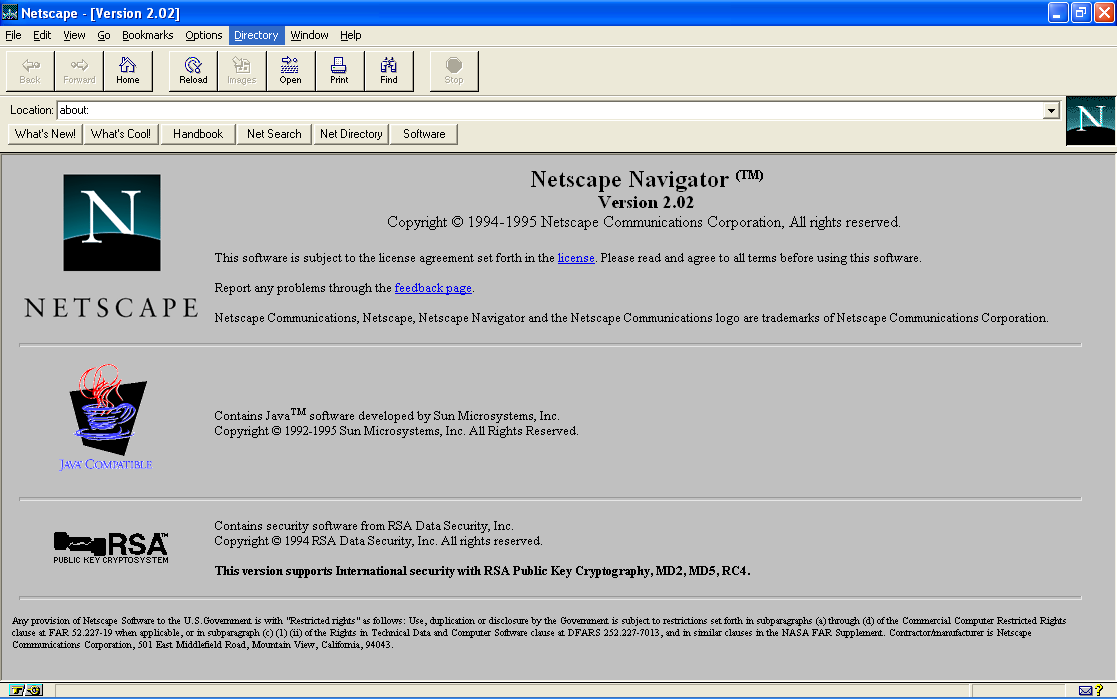
\includegraphics[width=400px]{Netscape_Navigator_2.png}
	\fonte{\citeonline{Softwsp2016netscape}}
	\label{fig:netscape}
\end{figure}

A Netscape enviou a linguagem para padronização à Associação Europeia de Fabricante de Computadores (ECMA) e devido a problemas de marca registrada, a versão padronizada da linguagem estava presa com o nome estranho “ECMAScript”. Pelos mesmos motivos de marca registrada, a versão da Microsoft da linguagem É formalmente conhecida como “JScript” \cite{flanagan2011javascript}.

O ECMAScript como foi padronizado não se destina a ser computacionalmente auto-suficiente, espera-se que o ambiente computacional de um programa ECMAScript forneça certos objetos específicos do ambiente; um navegador da Web fornece um ambiente de \emph{host} para computação do lado do cliente, incluindo, por exemplo, objetos que representam janelas, menus, pop-ups\footnote{Janela que abre no navegador da internet quando se acessa uma página na web ou algum link de redirecionamento.}, caixas de diálogo, áreas de texto, âncoras, quadros, histórico, cookies\footnote{Grupo de dados trocados entre o navegador e o servidor de páginas, colocado num arquivo de texto criado no computador do utilizador.} e entrada/saída; um servidor web fornece um ambiente de \emph{host} diferente para a computação do lado do servidor, incluindo objetos que representam requisições \cite{ecmascript2016}.

\subsection{Pré Ajax}

Em 1995, já era possível construir \emph{Single Page Applications} (SPAs) via frames/framesets\footnote{Divisões internas dentro de uma mesma janela do navegador, onde são carregados outros documentos HTML.} e url="javascript:...". Requisições assíncronas também eram possíveis utilizando JavaScript e manipulando elementos HTML que realizavam requisições HTTP; praticamente qualquer tag que possa ser configurado para fazer referência a um URL pode ser empregado para tarefas de comunicação com base em JavaScript \cite{powell2008ajax}.

Ainda segundo \citeonline{powell2008ajax}, utilizando-se de tags que referenciam URL é possível gerar uma requisição de via única ao servidor para indicar que algum evento aconteceu através de campos adicionados ao URL (\emph{Query Strings}). Para isso, utiliza-se de parâmetros passados via URL por uma tag\footnote{Estruturas de linguagem de marcação contendo instruções, tendo uma marca de início e outra de fim para que o navegador possa renderizar uma página.} (\emph{<img>} por exemplo), cabe ao servidor tratar a requisição e retornar o dado esperado ou uma resposta vazia com status 204, informando ao cliente que a solicitação ocorreu sem erros mas que não há conteúdo na resposta.

Quanto ao uso da tag \emph{<img>} para comunicação bi-direcional \citeonline{powell2008ajax} completa:

\begin{citacao}
	Parece que o uso de uma imagem provavelmente não é a melhor maneira de transmitir informações bidirecionais. Considere que, se você pedir uma imagem, você estará recebendo uma imagem, provavelmente em formato GIF, JPEG ou PNG para exibição. Como exemplo, você pode solicitar ao usuário alguns dados e, em seguida, gerar uma imagem personalizada para eles. A transmissão dos dados fornecidos pelo usuário é através da sequência de consulta como anteriormente, mas desta vez o servidor responderá não com um código 204, mas com uma imagem real para usar. Você pode usar o DOM e inseri-lo na página.
\end{citacao}

Visto que um navegador permanecerá na mesma página quando receber uma resposta HTTP de status 204, ele pode ser usado para fingir ir a uma URL apenas para enviar alguns dados; isto é feito em JavaScript com uma atribuição direta para \emph{window.location} enviando os dados pela URL, através das \emph{Query Strings}. Porem as \emph{Query Strings} são limitadas ao tamanho máximo da URL permitido pelo navegador.

Para envio de uma grande quantidade de dados o desenvolvedor precisaria realizar uma requisição HTTP POST com uma técnica de iframes\footnote{Elemento HTML que permite carregar as informações de um documento HTML separado em um documento HTML existente.} escondidos. Está técnica consiste da criação de campos de formulário a serem enviados com o formulário inserido no iframe. Uma vez que o formulário é preenchido com os dados desejados, é desencadeado o envio do formulário via JavaScript.

A utilização de iframe é flexível no que pode receber em comparação com alguns dos outros métodos, permitindo a comunicação bi-direcional através de respostas em XHTML\footnote{Linguagem Extensível para Marcação de Hipertexto.}, XML\footnote{Linguagem de marcação para a criação de documentos com dados organizados hierarquicamente.}, JSON\footnote{Notação de Objetos JavaScript, é uma formatação leve de troca de dados.} ou outro formato de codificação à serem tratado com JavaScript no navegador \cite{powell2008ajax}.

\subsection{Ajax}

O termo Ajax é um acrônimo para JavaScript assíncrono e XML que segundo \citeonline{Garrett2005}, descreve uma maneira de realizar uma comunicação HTTP a partir de uma aplicação JavaScript em páginas web.

Ajax é uma mistura do antigo com o novo, porque as tecnologias já existentes são combinadas em técnicas que pouco se considerava anteriormente, trazendo uma nova geração de aplicações é idéias \cite{gross2006introduction}.

Nesse contexto, \citeonline{Asleson2006} afirmam:
\begin{citacao}
	Honestamente, o Ajax não é nada novo. Na verdade, a tecnologia “mais nova” relacionada ao termo - o objeto XMLHttpRequest (XHR) - tem ocorrido desde o Internet Explorer 5 (lançado na primavera de 1999) como um controle ActiveX\footnote{Framework criado pela Microsoft que adapta as antigas versões das plataformas COM - Component Object Model e OLE - Object Linking and Embedding para conteúdo disponível online, especialmente aplicações web e cliente/servidor.}. No entanto, o que é novo é o nível de suporte do navegador. Originalmente, o objeto XHR era suportado apenas no Internet Explorer (limitando assim seu uso), mas, com o Mozilla 1.0 e Safari 1.2, o suporte é generalizado.
\end{citacao}

Criado pela Microsoft no fim da decada de 90, XMLHttpRequest é a interface através da qual o navegador pode fazer requisições HTTP com JavaScript. Quando a interface XMLHttpRequest foi adicionada ao Internet Explorer, ela permitiu que os desenvolvedores fizessem coisas com o JavaScript que antes era muito difícil \cite{haverbeke2014eloquent}.

Segundo \citeonline{grigorik2013high}, o XHR não apenas habilitou a comunicação assíncrona no navegador, mas também tornou mais simples esta, pois o XHR é uma API de aplicativos fornecida pelo navegador, o que significa que o navegador cuida automaticamente de todos os gerenciamentos de conexão de baixo nível.

Ainda segundo \citeonline{grigorik2013high}, o XHR tornou-se um padrão de fato em todos os principais navegadores porem o documento de especificação oficial só foi publicado em 2006 pelo \emph{World Wide Web Consortium} (W3C)\footnote{Principal organização de padronização da World Wide Web.}, bem depois de ter sido amplamente utilizado.

De fato, o envio de dados assíncronos ao servidor e a recepção de dados adicionais são o objetivo final do Ajax. Todos os processos do Ajax começam com uma conexão com o servidor. As conexões ao servidor geralmente são organizadas através do objeto XMLHttpRequest \cite{resig2007pro}.

\begin{figure}[!htb]
	\centering
	\caption{Comparação entre o modelo clássico e o modelo Ajax}
	\subfloat[Modelo clássico de aplicação WEB  (síncrono)]{
		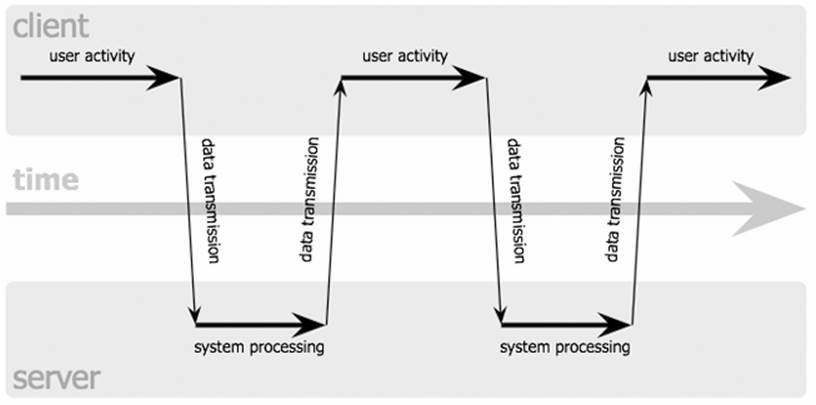
\includegraphics[width=210px]{default-pattern.jpg}
		\label{defaultPattern}
	}
	\hfill
	\subfloat[Modelo de aplicação WEB Ajax (assíncrono)]{
		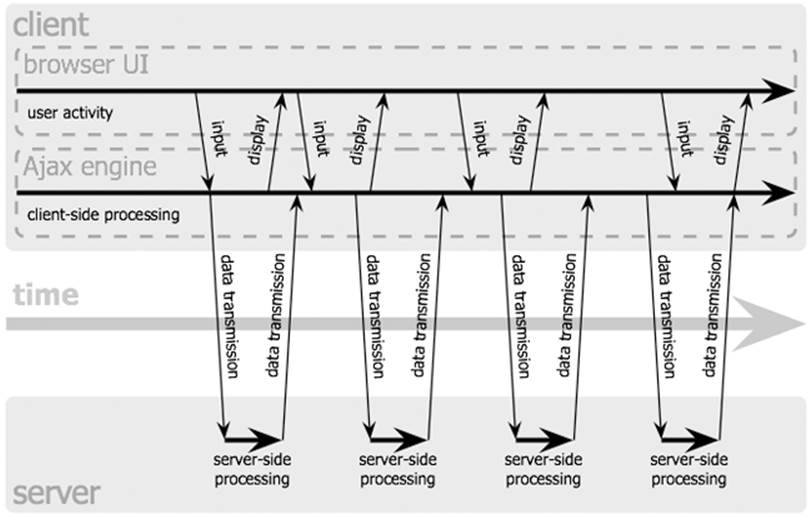
\includegraphics[width=210px]{ajax-pattern.png}
		\label{ajaxPattern}
	}
	\fonte{\citeonline{Garrett2005}}
	\label{defaultVsAjax}
\end{figure}

\begin{citacao}
	As versões iniciais do XHR proporcionaram recursos limitados: transferências de dados baseadas em texto, suporte restrito para o processamento de uploads e incapacidade de lidar com solicitações entre domínios\footnote{Nome que serve para localizar e identificar conjuntos de computadores na internet}. Para resolver essas falhas, o rascunho “XMLHttpRequest Level 2” foi publicado em 2008, que adicionou uma série de novos recursos \cite[P.~262-263]{grigorik2013high}.
\end{citacao}

Todos os novos recursos e recursos XHR2 são oferecidos através da mesma API XMLHttpRequest. Hoje, há apenas uma especificação XHR unificada, pois em 2011 a especificação “XMLHttpRequest Level 2” foi mesclada com a especificação original \cite{grigorik2013high}.

Uma lista de compatibilidade com os principais navegadores do mercado, pode ser conferida na Figura \ref{fig:xhr2}.

\begin{figure}[!htb]
	\centering
	\caption{Navegadores compatíveis com XHR2}
	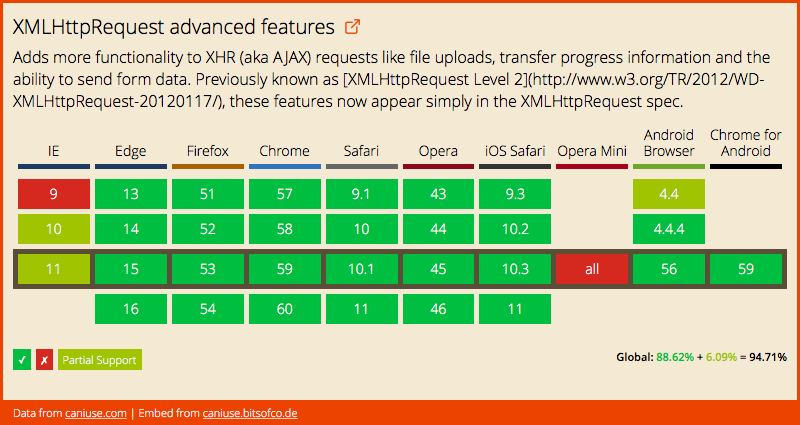
\includegraphics[width=400px]{XMLHttpRequest.png}
	\fonte{http://caniuse.com/\#feat=xhr2}
	\label{fig:xhr2}
\end{figure}

\subsection{HTTP Polling}

Segundo \citeonline[P.~273]{grigorik2013high}, “o HTTP não fornece nenhuma maneira para o servidor iniciar uma nova conexão com o cliente”. Para isso, o cliente deve pesquisar por atualizações no servidor.

Para uma atualização constante de informações entre o cliente e servidor, XHR nos fornece uma maneira simples. O cliente faz uma solicitação regular ao servidor solicitando atualizações e o servidor responde, podendo a resposta não conter dado. Esta técnica é conhecida por \emph{Polling HTTP} (ou \emph{Ajax Polling}). Tende a ser um desperdício de recursos de rede e de servidor, porem é fácil de implementar \cite{mccarthy2009comet}.

No entanto, de acordo com \citeonline{Pimentel2012}, \emph{Polling HTTP} é considerada uma boa solução para a entrega de informações em tempo real se o intervalo de entrega da mensagem for conhecido e  a taxa de transmissão de dados for constante. Porem, a cada consulta HTTP, repete-se informações de cabeçalho aumentando assim a latência.

Para reduzir a latência sem aumentar a carga do servidor, a solução é criar dois fluxos de comunicação entre o cliente e o servidor em uma técnica conhecida por \emph{Long Polling HTTP}. O primeiro fluxo é usado para receber mensagens e o segundo fluxo é usado para enviar mensagens. Para receber mensagens, o cliente pesquisa o servidor com um pedido de mensagens; se não houver mensagens, o servidor não responde com uma resposta imediatamente. O servidor coloca o pedido de pesquisa em espera por um período de tempo específico ou até que uma mensagem seja gerada pelo servidor  (Figura \ref{fig:longPolling}). A redução da latência é significativa ao converter o tempo inoperante em uma espera criada pelo servidor, enquanto o cliente aguarda o potencial de uma mensagem que está sendo gerada \cite{gross2006introduction}.

\begin{figure}[!htb]
	\centering
	\caption{Long Polling HTTP}
	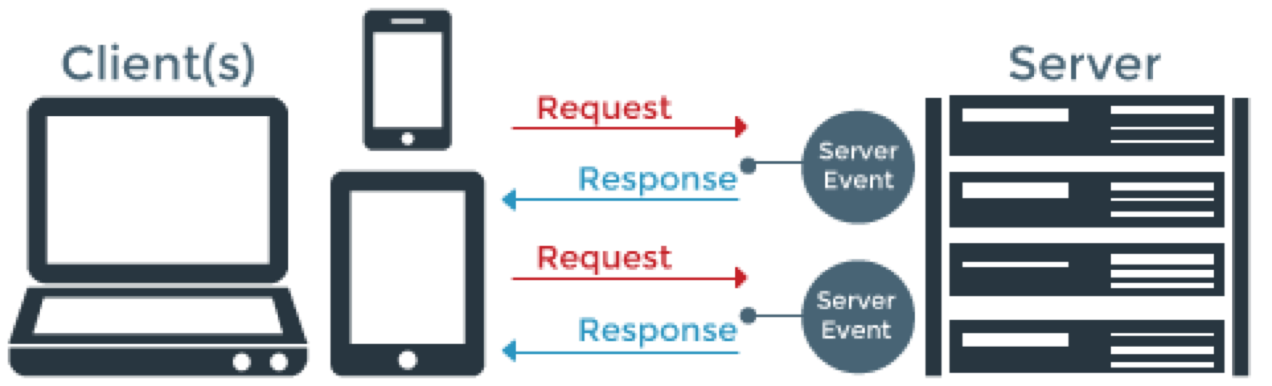
\includegraphics[width=400px]{Long-Polling.png}
	\fonte{\citeonline{Hanson2014long}}
	\label{fig:longPolling}
\end{figure}

Ainda segundo \citeonline{gross2006introduction}, o principal problema desta abordagem é que milhares de threads\footnote{Pequeno programa que trabalha como um subsistema, sendo uma forma de um processo se auto dividir em duas ou mais tarefas.} podem estar aguardando mensagens que possam ou não ser geradas, consumindo uma grande quantidade de Memória RAM\footnote{Tecnologia que permite o acesso aos arquivos armazenados no computador, responsável pela leitura dos conteúdos quando requeridos.}.

Nesta técnica, a conexão entre o cliente e servidor fica ociosa até expirar ou até que o servidor tenha dados para enviar. Cabe ao cliente a responsabilidade pela reconexão para aguardar a próxima atualização. Esta técnica é mais eficiente que \emph{Ajax Polling}, quando os dados são enviados com pouca frequência \cite{gutwin2011real}.

\subsection{HTTP Streaming}

Esta técnica se aproveita de um tipo de conteúdo HTTP chamado “\emph{multipart}” que permite que um servidor web envie conteúdo para um navegador em várias partes (\emph{chunked encoding}), projetada para o carregamento incremental de documentos muito grandes \cite{gutwin2011real}.

A implementação mais simples desta técnica é conhecida por \emph{ForeverFrame}, onde tem-se um iframe dentro de uma página HTML recebendo atualizações constantes através do recebimento de partes de dados contendo uma mensagem completa em cada parte. Inicialmente esta técnica foi bastante condenada no Internet Explorer, pois este trata cada fragmento recebido como uma carga de página, disparando então, som de clique do carregamento de página. A solução veio com a utilização do objeto \emph{htmlfile}\footnote{Interface para obter informações, examinar e modificar documentos HTML.} do ActiveX, tornando a técnica bastante popular \cite{souders2009even}.

Esta técnica também pode ser explorada em uma requisição XHR (\emph{XHR Streaming}), permitindo que um servidor web envie conteúdo para um navegador em várias partes. Essencialmente, o navegador é enganado para manter a conexão do soquete aberta, com o servidor enviando cada atualização como parte de um todo. O uso de uma única conexão de soquete também reduz o número de cabeçalhos HTTP que precisam ser enviados para pedidos e respostas, reduzindo assim, a latência \cite{gutwin2011real}.

Porem, se uma requisição \emph{XHR Streaming} continuar aberta por muito tempo, o navegador pode sofrer com o acumulo excessivo de memória RAM. No entanto, isto pode ser corrigido facilmente, simplesmente terminando a requisição e criando uma nova solicitação em um período de tempo definido ou após certa quantidade de mensagens recebidas \cite{souders2009even}.

\subsection{Server-Sent Event (SSE)}

Proposto desde 2009, define uma API para abrir uma conexão HTTP para receber notificações \emph{push}\footnote{Sistema de distribuição de conteúdo da Internet em que a informação sai de um servidor para um cliente, com base em uma série de parâmetros estabelecidos pelo cliente.} de um servidor na forma de eventos DOM, permitindo que os servidores enviem dados para páginas da Web por meio de HTTP ou usando protocolos dedicados de envio \cite{hicksonserver2015}.

Normatizado pelo W3C em fevereiro de 2015, apresenta a interface \emph{EventSource}; é projetada de modo que possa ser estendida para funcionar com outros esquemas de notificação \emph{push}, como \emph{Push SMS}\footnote{Serviço utilizado para o envio de mensagens de texto curtos, através de telefones celulares.} \cite{hicksonserver2015}.

\begin{citacao}
	Sob o capô, SSE oferece uma implementação eficiente e cruzada do \emph{XHR Streaming}; A entrega real das mensagens é feita através de uma única conexão HTTP de longa duração. No entanto, ao contrário de lidar com transmissão de XHR por conta própria, o navegador lida com todo o gerenciamento de conexão e análise de mensagens, permitindo que nossos aplicativos se concentrem na lógica de negócios! Em suma, a SSE torna o trabalho com dados em tempo real simples e eficiente \cite[P.~279]{grigorik2013high}.
\end{citacao}

Suportado nativamente pela maioria dos navegadores modernos (vide Figura \ref{fig:sse}); foi uma adição antecipada à especificação HTML5. No entanto, a interface \emph{EventSource} é simples, de modo que pode ser emulada através de uma biblioteca de JavaScript opcional (\emph{Polyfill}\footnote{Biblioteca JavaScript que implementa o padrão HTML5, quer seja um padrão estabelecido para todos os navegadores ou não.}) para navegadores que não o suportam nativamente \cite{grigorik2013high}.

\begin{figure}[!htb]
	\centering
	\caption{Navegadores compatíveis com Server-Sent Event}
	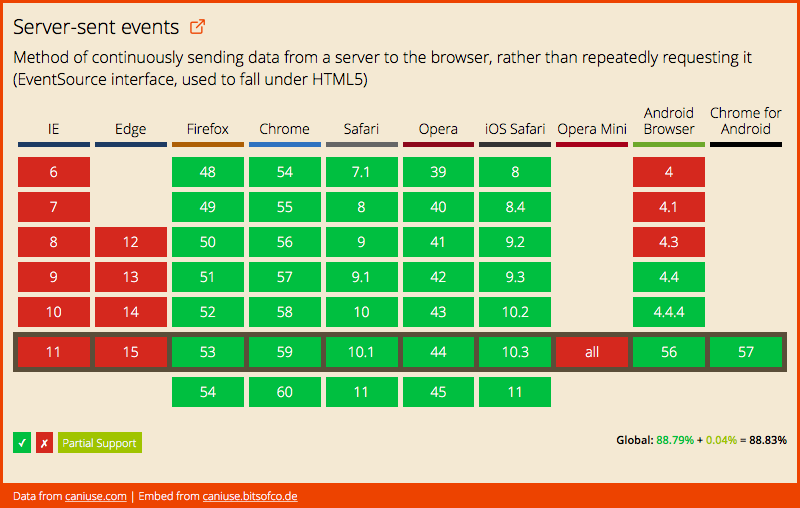
\includegraphics[width=400px]{Can_I_Use-SSE.png}
	\fonte{http://caniuse.com/\#feat=eventsource}
	\label{fig:sse}
\end{figure}

\subsection{WebSockets}



\section{CONCLUSÃO}

% Este tópico trata da recapitulação sintética dos resultados da pesquisa, do alcance e as suas contribuições, bem como seu possível mérito. Deve ser breve e basear-se em dados comprovados.

% TODO: Fazer a conclusão

%Em última análise, todos esses métodos para fornecer dados em tempo real envolvem cabeçalhos de solicitação HTTP e resposta, que contêm muitos dados de cabeçalho adicionais e desnecessários e apresentam latência. Além disso, a conectividade full-duplex requer mais do que apenas a conexão a jusante do servidor para o cliente. Em um esforço para simular a comunicação full-duplex em HTTP half-duplex, muitas das soluções de hoje usam duas conexões: uma para downstream e outra para upstream. A manutenção e coordenação destas duas conexões introduz altos custos gerais em termos de consumo de recursos e acrescenta muita complexidade. Simplificando, o HTTP não foi projetado para comunicação full-duplex em tempo real como você pode ver na Figura 7-1, que mostra as complexidades associadas à construção de um aplicativo da Web que exibe dados em tempo real a partir de dados de back-end Fonte usando um modelo de publicação / assinatura sobre HTTP half-duplex \cite{lubbers2011pro}.

%É ainda pior quando tenta dimensionar essas soluções. Simular a comunicação do navegador bidirecional através de HTTP é propenso a erros e complexo e toda essa complexidade não escala. Mesmo que seus usuários finais possam estar desfrutando de algo que se parece com uma aplicação web em tempo real, essa experiência "em tempo real" tem um preço alto. É um preço que você pagará em latência adicional, tráfego de rede desnecessário e um arrasto no desempenho da CPU \cite{lubbers2011pro}.

{ \clearpage
	\bibliography{./src/referencias}
}

%{ \clearpage
	%\listoftables
%}

{ \clearpage
	\listoffigures
}

\end{document}

% TODO: verificar se precisa de numeração de páginas
